\subsection{PatternNet and PatterAttribution}
Using either a simple linear model~\cite{Kindermans.2018} or a constant shift in mean~\cite{Kindermans.2019}, \citeauthor{Kindermans.2018} were able to show the vulnerability of gradient methods (such as \gls{lrp}, \gls{td}, \gls{dtd}, Gradient x Input, and Integrated Gradients) to random changes in the input-sample (see \cref{fig:kindermans-unreliability}).
\begin{figure*}
    \center{}
    \includegraphics[width=\textwidth]{kindermans-catastrophic-attribution}
    \caption[Evaluation of attribution methods via a constant shift on MNIST]{Evaluation of attribution methods on two models (Network 1 and Network 2). Network 1 is trained on the well known MNIST-Dataset, while Network 2 is trained on a manipulated Version of MNIST with a constant shift (i.e. a hand-drawn image of a cat). Because the constant shift does not add any information to an image, a consistent attribution method should provide a similar explanation for both Network 1 and Network 2, when applied to the same input image with only the constant shift. However, Gradient x Input, Integrated Gradients and \gls{lrp} show a difference between Network 1 and Network 2. For further details, refer to~\cite{Kindermans.2019} from where this figure was adopted.}
    \label{fig:kindermans-unreliability}
\end{figure*}
To overcome this vulnerability of preexisting methods, \fcite{Kindermans.2018} introduce \textit{signal estimators} \(S(x)\) that will be explained in this subsection. Signal estimators root in the idea that each input-sample \(x\) of a dataset is a combination of underlying signal \(s\) (contains all information about e.g.\ the correct class) and distractor \(d\) (does not contain any information about e.g\ the correct class) such that \(x=s\circ d\), with \(\circ\) being some operation, for simplicity let \(\circ\) denote summation \(\circ:=+\)~\cite{Kindermans.2018}. A signal estimator \(S(x)\) is then used to extract \(d\) from \(x\), such that for an optimal signal estimator: \(s = x - S(x)\).
\begin{description}
    \item[\namedlabel{itm:sw-signal-estimator}{The Filter-Based Estimator \(\symbfit{S_w}\)}{\(\symbfit{S_w}\)}] is equal to the \ref{itm:w2weighting} discussed in \cref{subsect:dtd}.
    \begin{equation}
        S_w = \frac{w_{ij}^2}{\sum_{h\in (l)} w_{hj}^2}.
    \end{equation}
    Although simple, \fcite{Kindermans.2018} show that \(S_w(x)\) neither holds theoretically, being unable to separate \(s\) and \(d\), nor empirically as shown in \cref{fig:kindermans-signal-estimator-comparison}.
    \item[\namedlabel{itm:sa-signal-estimator}{The Linear Estimator {}\(\symbfit{S_a}\)}{\(\symbfit{S_a}\)}] is based on the assumption of a linear perceptron. Although this assumptions does not even hold for simple ReLU's, it provides a significant improvement over \ref{itm:sw-signal-estimator} as shown in \cref{fig:kindermans-signal-estimator-comparison}.
    \begin{equation}
        S_{a(i)}(x) = x_{(i)} (a_{(i)} w_{ij})\label{eq:linear-estimator}
    \end{equation}
    please note that, while the weights \(w_{ij}\), which are taken from a trained model, and the input-variable of the input-sample \(x_{(i)}\) are fixed parameters, \(a_{(i)}\) must be trained on a given dataset. Details on the training are provided in~\cite{Kindermans.2018}. \Cref{eq:linear-estimator} is an exemplary formulation of \(S_a\) for the input layer.
    \item[\namedlabel{itm:sa+-signal-estimator}{The Two-Component Estimator \(\symbfit{S_{a+-}}\)}{\(\symbfit{S_{a+-}}\)}] is tailored to ReLU-activation functions. \fcite{Kindermans.2018} notice that due to applying ReLU's, the weights used in previous signal estimators \ref{itm:sw-signal-estimator}, \ref{itm:sa-signal-estimator} are only trained on positive signal \(s_{+}\) and distractor \(d_{+}\) values. To account also for negative \(s_{-}, d_{-}\), they split the estimator accordingly
    \begin{equation}
        S_{a+-(i)} = 
        \begin{cases}
            x_{(i)} (a_{+(i)} w_{ij}),& {\scriptstyle \text{if } (x_{(i)} w_{ij}) > 0}\\
            x_{(i)} (a_{-(i)} w_{ij}),& {\scriptstyle \text{otherwise}}
        \end{cases}
    \end{equation}
    again note that, while the weights \(w_{ij}\) and the input-variable \(x_{(i)}\) are fixed parameters, \(a_{+(i)}, a_{-(i)}\) must be trained on a given dataset. Details on the training are provided in~\cite{Kindermans.2018}.
\end{description}\label{desc:signal-estimators}
\par
In summary, \citeauthor{Kindermans.2018} propose 
\begin{enumerate*}[label={\roman*)}]
    \item the concept of signal estimators in order to overcome the vulnerability of previous methods to a constant-shift in the input and
    \item two new signal estimators, \ref{itm:sa-signal-estimator} and \ref{itm:sa+-signal-estimator}, which significantly improve upon the previously (and naively) used estimator \ref{itm:sw-signal-estimator}.
\end{enumerate*} A visual example for the three signal estimators is provided in \cref{fig:kindermans-signal-estimator-visually}.
\par
For \textit{PatternAttribution}, \fcite{Kindermans.2018} then use the derived signal estimator as a weighting parameter in the \gls{dtd}-framework, which can be interpreted as an informed choice of root-point \(x_0\).
For \textit{PatternNet}, only the signal itself is reconstructed.\todo{sHOw aN iMaGE oF THiS}
\begin{figure*}[ht]
    \center{}
    \includegraphics[width=\textwidth]{kindermans-signal-estimators}
    \caption[Evaluation of Signal Estimators for VGG-16 on different layers.]{Evaluation of Signal Estimators for VGG-16 on different layers. Higher values are better. A random Signal Estimator is used as baseline. For details on the quality measure \(\rho\) refer to \cite{Kindermans.2018} from where this figure was adopted.}
    \label{fig:kindermans-signal-estimator-comparison}
\end{figure*}
\begin{figure}
    \center{}
    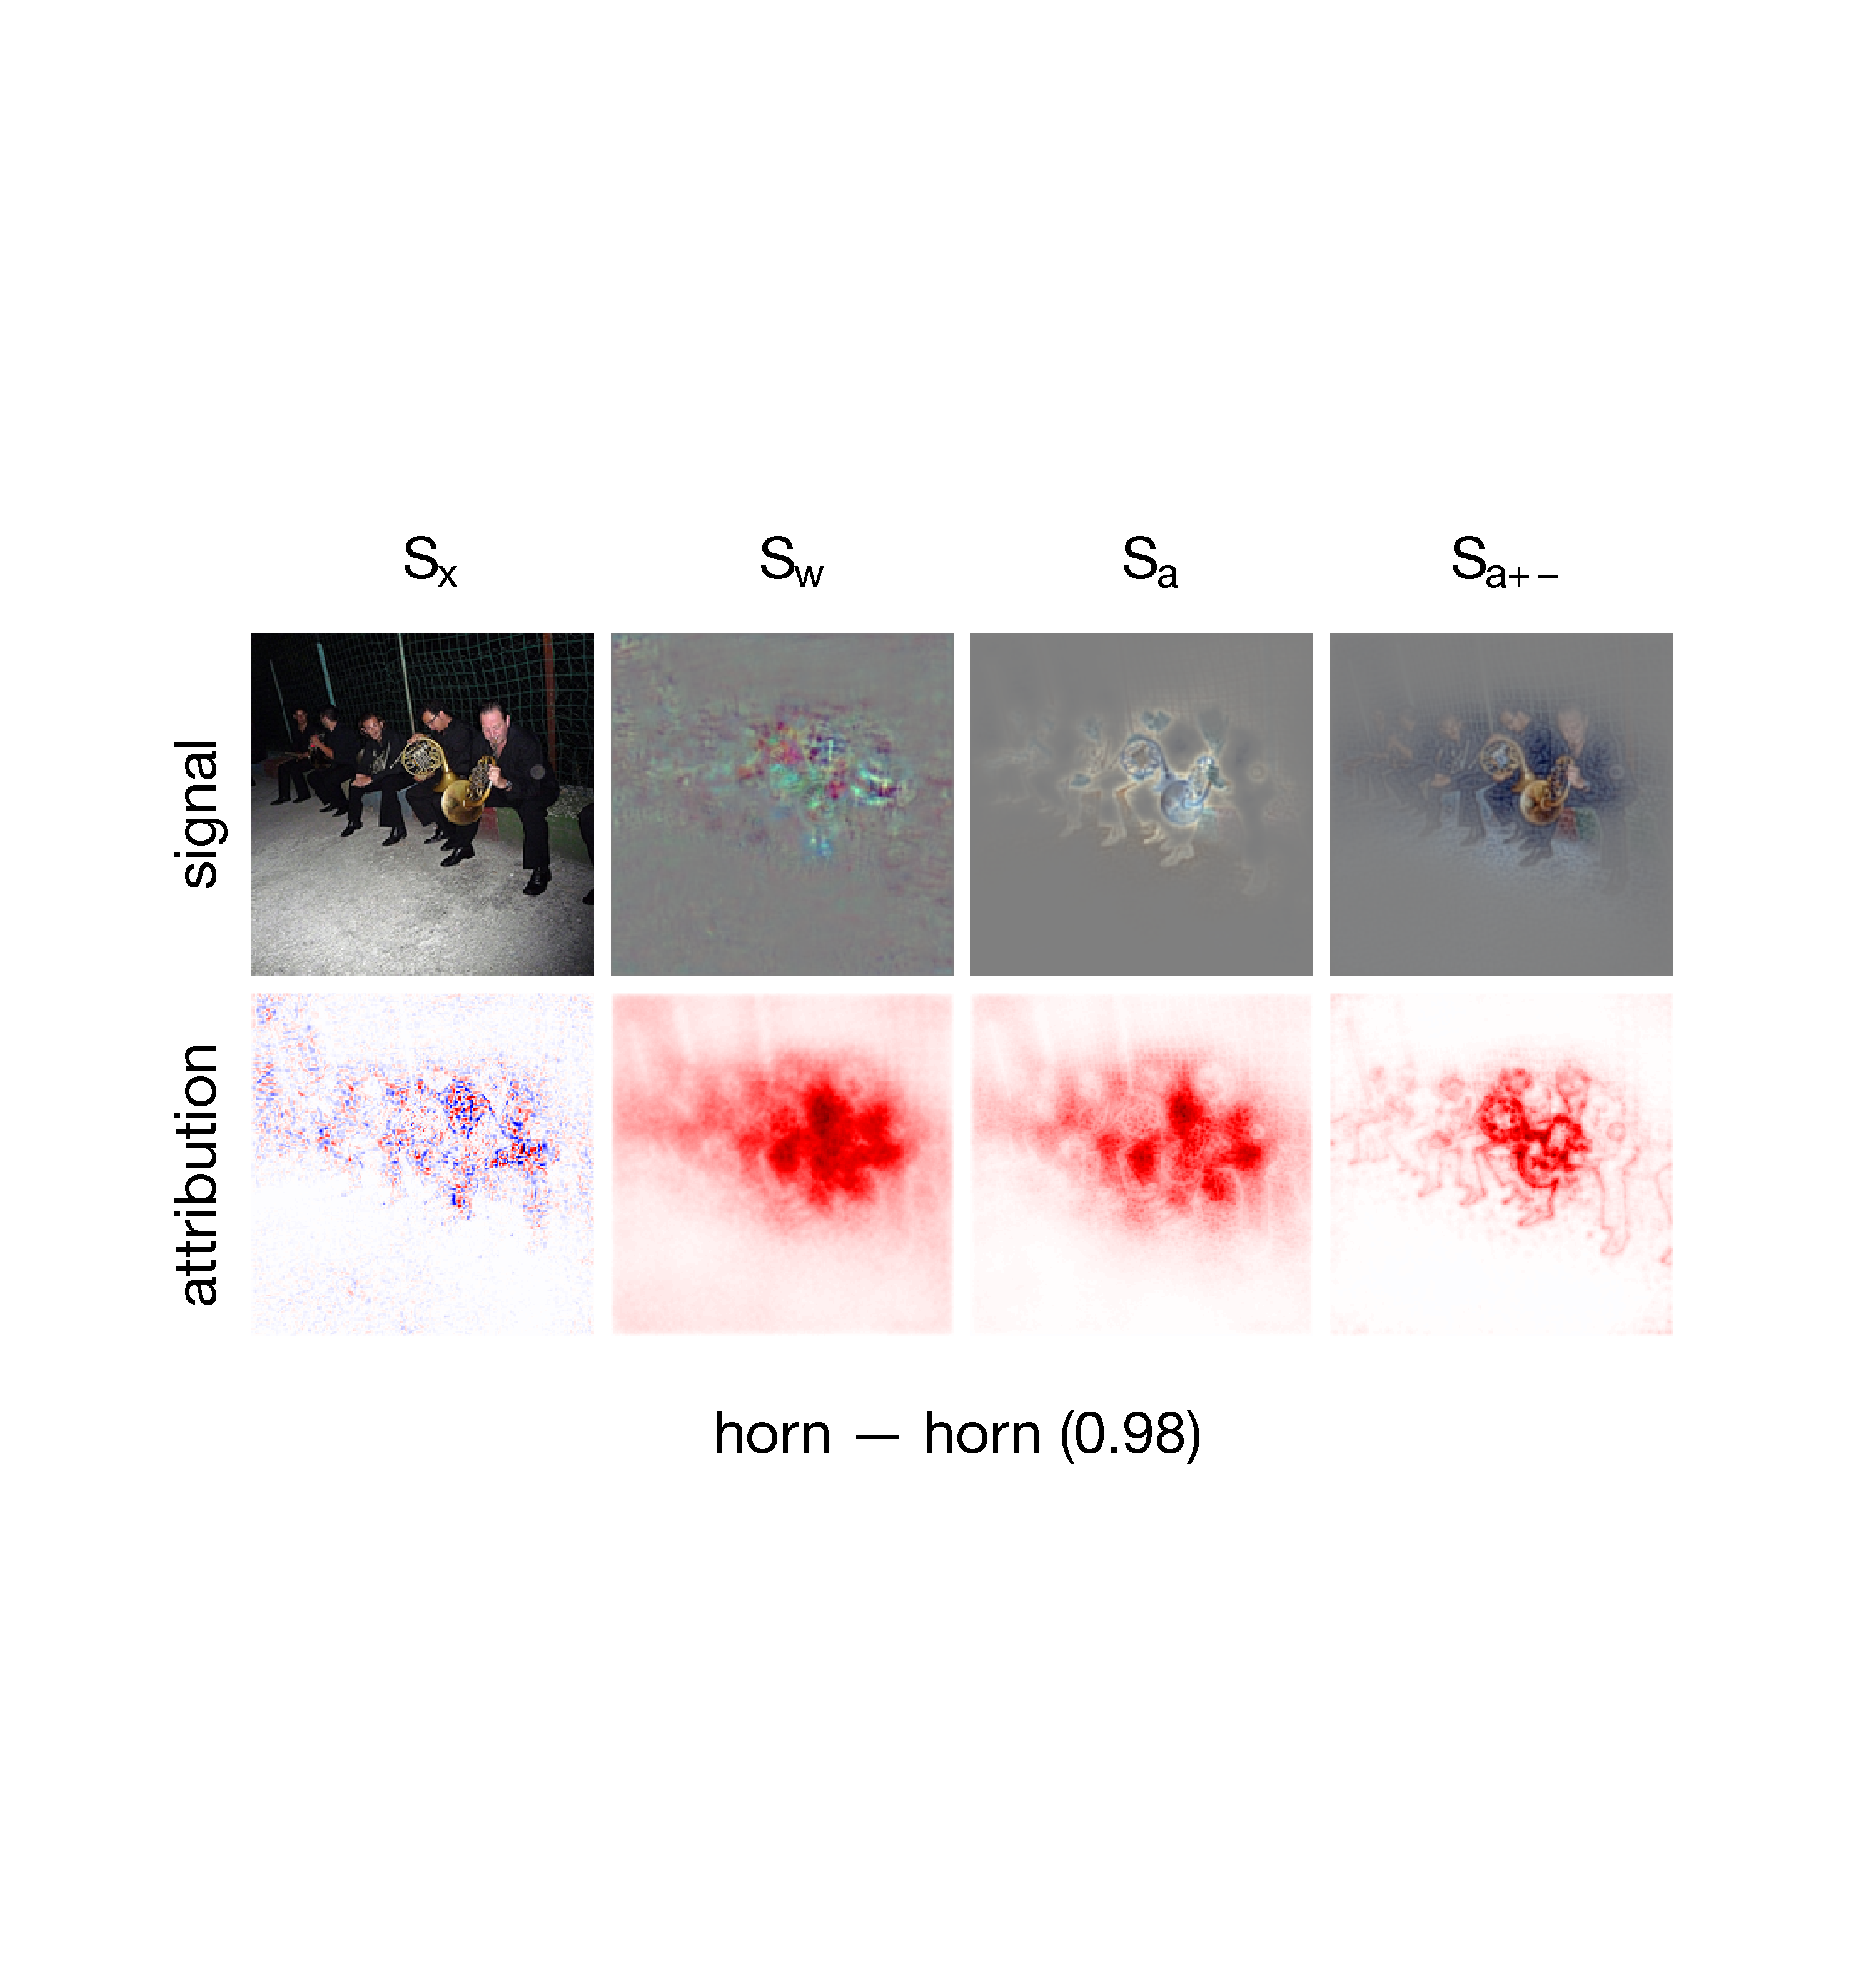
\includegraphics[width=\textwidth/2]{kindermans-signal-estimators-visually}
    \caption[Visual example for the three signal estimators.]{Visual example for the three signal estimators. \(S_x\) is the identity estimator with \(S_x(x)=x\). Figure adopted from~\cite{Kindermans.2018}}\label{fig:kindermans-signal-estimator-visually}
\end{figure}